\documentclass[a4paper,11pt]{book}
%\documentclass[a4paper,twoside,11pt,titlepage]{book}
\usepackage{array}
\usepackage{cite}
\usepackage{dirtree}
\usepackage{listings}
\usepackage{longtable}
\usepackage{float}
\usepackage{subfig}
\usepackage{url}
\usepackage[utf8]{inputenc}
\usepackage[spanish]{babel}
\usepackage[sort&compress]{natbib}
% \usepackage[style=list, number=none]{glossary} %
%\usepackage{titlesec}
%\usepackage{pailatino}

\decimalpoint
\usepackage{dcolumn}
\newcolumntype{.}{D{.}{\esperiod}{-1}}
\makeatletter
\addto\shorthandsspanish{\let\esperiod\es@period@code}
\makeatother


%\usepackage[chapter]{algorithm}
\RequirePackage{verbatim}
%\RequirePackage[Glenn]{fncychap}
\usepackage{fancyhdr}
\usepackage{graphicx}
\usepackage{afterpage}

\usepackage{longtable}

\usepackage[pdfborder={000}]{hyperref} %referencia

% ********************************************************************
% Re-usable information
% ********************************************************************
\newcommand{\myTitle}{Desarrollo de un simulador de escenarios con usuarios móviles para la evaluación de algoritmos de recomendaciones}
\newcommand{\myDegree}{GRADO EN INGENIERÍA INFORMÁTICA}
\newcommand{\TFG}{TRABAJO FIN DE GRADO}
\newcommand{\myName}{Slavcho Georgiev Ivanov}
\newcommand{\myProf}{Sergio Ilarri Artigas}
\newcommand{\myFaculty}{Escuela de Ingeniería y Arquitectura}
\newcommand{\myFacultyShort}{EINA}
\newcommand{\myArea}{Área de Lenguajes y Sistemas Informáticos}
\newcommand{\myDepartment}{Departamento de Informática e Ingeniería de Sistemas}
\newcommand{\myUni}{\protect{Universidad de Zaragoza}}
\newcommand{\myLocation}{Zaragoza}
\newcommand{\myTime}{\today}
\newcommand{\myVersion}{Version 0.1}


\hypersetup{
pdfauthor = {\myName (email (en) ugr (punto) es)},
pdftitle = {\myTitle},
pdfsubject = {},
pdfkeywords = {palabra_clave1, palabra_clave2, palabra_clave3, ...},
pdfcreator = {LaTeX con el paquete ....},
pdfproducer = {pdflatex}
}

\usepackage{url}
\usepackage{colortbl,longtable}
\usepackage[stable]{footmisc}

\pagestyle{fancy}
\fancyhf{}
\fancyhead[LO]{\leftmark}
\fancyhead[RE]{\rightmark}
\fancyhead[RO,LE]{\textbf{\thepage}}
\renewcommand{\chaptermark}[1]{\markboth{\textbf{#1}}{}}
\renewcommand{\sectionmark}[1]{\markright{\textbf{\thesection. #1}}}

\setlength{\headheight}{1.5\headheight}

\newcommand{\HRule}{\rule{\linewidth}{0.5mm}}
%Definimos los tipos teorema, ejemplo y definición podremos usar estos tipos
%simplemente poniendo \begin{teorema} \end{teorema} ...
\newtheorem{teorema}{Teorema}[chapter]
\newtheorem{ejemplo}{Ejemplo}[chapter]
\newtheorem{definicion}{Definición}[chapter]

\definecolor{gray97}{gray}{.97}
\definecolor{gray75}{gray}{.75}
\definecolor{gray45}{gray}{.45}
\definecolor{gray30}{gray}{.94}

\lstset{ frame=Ltb,
     framerule=0.5pt,
     aboveskip=0.5cm,
     framextopmargin=3pt,
     framexbottommargin=3pt,
     framexleftmargin=0.1cm,
     framesep=0pt,
     rulesep=.4pt,
     backgroundcolor=\color{gray97},
     rulesepcolor=\color{black},
     %
     stringstyle=\ttfamily,
     showstringspaces = false,
     basicstyle=\scriptsize\ttfamily,
     commentstyle=\color{gray45},
     keywordstyle=\bfseries,
     %
     numbers=left,
     numbersep=6pt,
     numberstyle=\tiny,
     numberfirstline = false,
     breaklines=true,
   }
 
% minimizar fragmentado de listados
\lstnewenvironment{listing}[1][]
   {\lstset{#1}\pagebreak[0]}{\pagebreak[0]}

\lstdefinestyle{CodigoC}
   {
	basicstyle=\scriptsize,
	frame=single,
	language=C,
	numbers=left
   }
\lstdefinestyle{CodigoC++}
   {
	basicstyle=\small,
	frame=single,
	backgroundcolor=\color{gray30},
	language=C++,
	numbers=left
   }

 
\lstdefinestyle{Consola}
   {basicstyle=\scriptsize\bf\ttfamily,
    backgroundcolor=\color{gray30},
    frame=single,
    numbers=none
   }


\newcommand{\bigrule}{\titlerule[0.5mm]}


%Para conseguir que en las páginas en blanco no ponga cabecerass
\makeatletter
\def\clearpage{%
  \ifvmode
    \ifnum \@dbltopnum =\m@ne
      \ifdim \pagetotal <\topskip
        \hbox{}
      \fi
    \fi
  \fi
  \newpage
  \thispagestyle{empty}
  \write\m@ne{}
  \vbox{}
  \penalty -\@Mi
}
\makeatother

\usepackage{pdfpages}
\begin{document}
\begin{titlepage}
 
 
\newlength{\centeroffset}
\setlength{\centeroffset}{-0.5\oddsidemargin}
\addtolength{\centeroffset}{0.5\evensidemargin}
\thispagestyle{empty}

\noindent\hspace*{\centeroffset}\begin{minipage}{\textwidth}

\centering

\includegraphics[width=0.9\textwidth]{imagenes/diislogoblanco_0.png}\\[1.4cm]

\textsc{ \Large TRABAJO FIN DE GRADO\\[0.2cm]}
\textsc{ GRADO EN INGENIERÍA INFORMÁTICA}\\[1cm]
% Upper part of the page
% 
% Title
{\Huge\bfseries Simulador de escenarios con usuarios móviles\\
}
\noindent\rule[-1ex]{\textwidth}{3pt}\\[3.5ex]
%{\large\bfseries Subtitulo del Proyecto}
\end{minipage}

\vspace{2.5cm}
\noindent\hspace*{\centeroffset}\begin{minipage}{\textwidth}
\centering

\textbf{Autor}\\ {Slavcho Georgiev Ivanov}\\[2.5ex]
\textbf{Director}\\
{Sergio Ilarri Artigas}\\[2cm]

\includegraphics[width=0.3\textwidth]{imagenes/logo-eina.png}\\[0.1cm]
\textsc{Escuela de Ingeniería y Arquitectura}\\
\textsc{Área de Lenguajes y Sistemas Informáticos}\\
\textsc{Departamento de Informática e Ingeniería de Sistemas}\\
\textsc{---}\\
Zaragoza, Julio de 2016
\end{minipage}
%\addtolength{\textwidth}{\centeroffset}
%\vspace{\stretch{2}}
\end{titlepage}



\chapter*{}

\cleardoublepage
\thispagestyle{empty}

\begin{center}
{\large\bfseries \myTitle}\\
\end{center}

\vspace{0.7cm}
\noindent{\textbf{Resumen}}\\

Los sistemas de recomendación proporcionan sugerencias acerca de elementos que pueden resultar de interés para el usuario como pueden ser los hoteles, restaurantes, libros, películas, lineas de taxis y autobuses etc. Habitualmente estos sistemas se evalúan con conjuntos de datos estáticos clásicos pero el inconveniente que esto conlleva es que solo podemos realizar un análisis sobre el comportamiento de los usuarios en el pasado perdiendo la capacidad de poder calibrar correctamente los algoritmos de recomendaciones para su correcta evaluación.

El objetivo de este Trabajo Fin de Grado es desarrollar un simulador de escenarios con usuarios móviles que recolecte y proporciones conjuntos de datos dinámicos para la evaluación de algoritmos de recomendaciones. 

La arquitectura del sistema consta de un navegador web, un servidor web Node.js, un servidor de recomendaciones y una base de datos mongoDB. Se trata de una aplicación web de una sola página desarrollada con Angular.js y Node.js que nos permite configurar distintos escenarios con conjuntos de datos reales obtenidos a partir del servicio de mapas de OpenStreetMap.

La integración entre los distintos componentes del sistemas está realizada de dos maneras. La primera es una REST API y el intercambio de mensajería JSON para realizar operaciones de tipo CRUD para las distintas configuraciones del simulador y la segunda es un sistema bidireccional dirigido por eventos utilizado durante las simulaciones para compartir información entre los distintos componentes del sistema sin que estos la hayan solicitado evitando mucha peticiones innecesarias y consiguiendo que las simulaciones funcionen en tiempo real.

Para la gestión del proyecto se ha elegido el modelo en espiral como modelo de trabajo. Esto me ha permitido evaluar los requisitos en cada iteración y reorientar el proyecto al encontrar dificultados y limitaciones.

\cleardoublepage


\thispagestyle{empty}


\chapter*{Agradecimientos}
\thispagestyle{empty}

       \vspace{1cm}


Me gustaría agradecer este Trabajo Fin de Grado a todas las personas que lo han echo posible con su apoyo y dedicación.

\vspace{1cm}
En su primer lugar a mi director Sergio Ilarri por la oportunidad que me ha dado para realizar este proyecto, su paciencia y ayuda, sin la cual este proyecto no hubiera sido posible. A mis compañeros y amigos de clase, con los que he compartido estos años de carrera, por hacer que los momentos de estudio y prácticas fuesen agradables y amenos. A mi familia y amigos más cercanos, por su paciencia y por motivarme para seguir adelante en los momentos más complicados.

\vspace{1cm}
Y por supuesto a la Universidad de Zaragoza y a todos aquellos profesores de lo que he aprendido tanto a los largo de estos años.

\cleardoublepage

\frontmatter
\tableofcontents
\listoffigures
\listoftables

%
\mainmatter
\setlength{\parskip}{5pt}

\chapter{Introducción}

En este capítulo se mostrará la motivación existente para la realización de este Trabajo Fin de Grado, los objetivos que han sido marcados por el proyecto, las librerías y herramientas utilizadas para su elaboración, el modelo de trabajo seleccionado y también se analizará el contexto tecnológico. Finalmente se mostrará la estructura seguida en este documento.

\section{Motivación del proyecto}

Han sido varias las razones que me llevaron a elegir desarrollar este Trabajo Fin de Grado. La primera y principal ha sido el interés personal en los sistemas de recomendaciones y su amplia aplicación en sistemas comerciales y la web. Por otro lado, realizar un proyecto complejo, partiendo desde cero y sin tener ningún conocimiento particular de este ámbito, suponía un gran reto que deseaba afrontar porque me permitiría ampliar mis conocimientos en campos diversos como Ingeniería del Software, Arquitecturas de Software etc., de las que poseía unos conocimientos limitados. Además, consideré que la experiencia y conocimientos que adquiriría en este proyecto aumentarian mis posibilidades de desarrollar mi carrera profesional en este ámbito.

\section{Objetivos}

El Trabajo Fin de Grado que se describe en este documento tiene los siguientes objetivos:

\begin{itemize}
	\item Desarrollar un simulador de escenarios con usuarios móviles, que cuente con mapas de ciudades con objetos móviles y estáticos.
	\item Desarrollar lo necesario para que se permita que los mapas de ciudades sean reales de tal forma que estos sean obtenidos de un sistema que proporcione mapas.
       \item Desarrollar lo necesario para que los usuarios puedan crear, editar, borrar y configurar los mapas y escenarios del simulador.
       \item Desarrollar lo necesario para que todas las configuraciones de mapas y escenarios sean parametrizables desde la interfaz de usuario.
       \item Desarrollar lo necesario para que la simulación de escenas funcione en tiempo real de tal forma que los eventos de una escena se reflejen en los dispositivos de los usuarios conectados al mismo mapa y escena.
       \item Desarrollar una interfaz que permita la integración con un recomendador externo de tal forma que exista una comunición bidireccional basada en eventos entre el simulador y el recomendador.
\end{itemize}

Además de los objetivos marcados por la propuesta del Trabajo Fin de Grado, también se han tenido en cuenta como objetivos lograr que el simulador utilize los recursos hardware minimos, permitir que este sea facilmente escalable y que pueda desplegarse en un entorno distribuido. De esta forma logramos ahorar costes de infraestructura y futuros desarrollos.

\section{Contexto Tecnológico}

Habitualmente los sistemas de recomendación se evalúan con conjuntos de datos estáticos clásicos. El incoveniente que esto conlleva es que si ejecutamos el mismo algoritmo sobre un conjunto de datos estáticos varias veces siempre obtenemos el mismo resultado. Con el fin de evitar este incoveniente surge la necesidad de evaluar los algoritmos de recomendaciones con conjuntos de datos dinámicos. 

Una de las formas de recolectar y proveer conjuntos de datos dinámicos es mediante el crowdsourcing. El crowdsourcing, tambien conocido como colaboración abierta distribuida, consiste en delegar tareas a un grupo de personas o comunidad a través de una convocatoria abierta. 

Así que a medida que el grupo de personas o comunidad vayan realizando las tareas asignadas el sistema va recolectado y suministrando datos sobre las acciones que realizan estos para llevar a cabo sus tareas. Esto nos da la oportunidad para suministrar datos a los algoritmos de recomendaciones en tiempo real, es decir, suministrar datos a medida que el grupo de personas vayan cumpliendo con sus tareas.   

\section{Herramientas utilizadas}

En esta sección se listan las tecnologias, libererías externas y herramientas utilizadas para el desarrollo del proyecto acompañada de una breve descripción.

\noindent{\textbf{Librerías usadas}}\\

Para el desarrollo del proyecto se ha hecho uso de diversas librerías externas que han permitido la implementación en un tiempo razonable de ciertas funciones necesarias que no formaban parte de los objetivos del proyecto:

\begin{itemize}
       \item {\bfseries Openlayers}: framework de OpenStreetMap que nos permite el uso libre de mapas.
       \item {\bfseries Node.js v0.12.4}: entorno Javascript del lado del servidor basado en el motor V8 de Google. 
       \item {\bfseries Express v4.12.4}: framework de Node.js destinado a la creación de APIs Rest
       \item {\bfseries Angular.js}: framework javascript que facilita la creación de aplicaciones en una sola página. 
       \item {\bfseries Mongoose v4.1.2}: framework de Node.js destinado al modelado de objetos para MongoDB.
       \item {\bfseries jwt.io v5.0.4}: framework destinado a la creación y distribución de web tokens. 
       \item {\bfseries socket.io v1.4.4}: framework de Node.js destinado a la creación de comunicaciones bidirecionales basadas en eventos
       \item {\bfseries Apache mahout v0.11.1}: framework de Java destinado al aprendizaje automático.
       \item {\bfseries socket.io-client v0.1.0}: cliente Java para socket.io desarrollado por Naoyuki Kanezawa
\end{itemize}

\newpage       
\noindent{\textbf{Herramienta de desarrollo}}\\

Durante el desarrollo de este Trabajo Fin de Grado se han utilizado las siguientes herramientas:

\begin{itemize}
       \item {\bfseries Eclipse Java EE IDE}: editor de código Java version Mars 4.5.1
       \item {\bfseries Maven v3.2.5}: gestor de paquetes para desarrollos Java
       \item {\bfseries Brackets.io v1.6.0}: editor de código para desarrollos web
       \item {\bfseries Git v1.9.4}: sistema de control de versiones
       \item {\bfseries GitHub}: repositorio de código
       \item {\bfseries Cmder}: emulador cmd de Windows 
       \item {\bfseries Sublime text 2}: editor de texto avanzado
       \item {\bfseries CityEngine 2014}: software de modelado de cuidades
       \item {\bfseries Unity 5}: motor gráfico para la creación de videojuegos
       \item {\bfseries OSM2Word}: visualizador de datos con formato OSM
\end{itemize}

\noindent{\textbf{Herramienta de documentación}}\\

Se han usado las siguientes herramientas para la elaboración de la documentación del proyecto:

\begin{itemize}
       \item {\bfseries Latex}: lenguaje usado para la elaboración de este documento
       \item {\bfseries GanttProject}: editor de diagramas de Gantt
       \item {\bfseries Gliffy Diagrams}: editor de multiples tipos de diagramas (daigramas de flujos, UML, etc.)
\end{itemize}


\section{Modelo de proceso seleccionado}

El modelo de trabajo seleccionado está basado en el modelo de espiral. Las actividades de este modelo forman una espiral de tal forma que cada iteración representa un conjunto de actividades. Se ha elegido este modelo de trabajo porque nos permitiría integrar el desarrollo con el mantenimiento y evaluar en cada iteración si dichos requisitos siguen encajando de lo que se esperaba de la aplicación para conseguir los objetivos propuestos. De esta forma se reduce el riesgo del proyecto y se incorporan objetivos de calidad.

\section{Estructura de la memoria}

El contenido de la memoría está distribuido de la siguiente forma:

\begin{itemize}
	\item En el capítulo 2 se expone el trabajo desarrollado para la elaboración de este simulador
	\item En el capítulo 3 se expone la gestión del proyecto y las distintas etapas por las que ha pasado este proyecto
	\item En el capítulo 4 se muestran las conclusione del proyecto y el posible trabajo futuro de cara a mejorar el simulador 
\end{itemize}
%
\chapter{Trabajo desarrollado}


En este capítulo se explican las funcionalidades básicas del simulador desarrollado centradose únicamente en los aspectos más importantes.

\section{Resumen del simulador}

El simulador RecSim permite representar escenarios adaptados a las necesidades de simulación existentes. Un escenario se compone de un mapa y de un conjunto de objetos, y puede definirse sobre cualquier mapa real existente en OpenStreetMap: el usuario puede utilizar un buscador para ver un mapa y luego seleccionar dentro de dicho mapa el área geográfica de interés. Además, se pueden definir tipos de objetos estáticos (por ejemplo, restaurantes, hoteles, cines, etc.) y tipos de objetos dinámicos o móviles (por ejemplo, taxis, buses,ambulancias, etc.), asociándoles un nombre de tipo y un icono que se utilizará para representar instancias de dicho tipo de objeto en un mapa. Luego pueden colocarse en un escenario objetos estáticos y dinámicos de los tipos deseados: los objetos estáticos se colocan en la posición deseada sobre el mapa y a los objetos dinámicos se les asigna una determinada trayectoria o un comportamiento de movimientos aleatorios. Alternativamente, pueden importarse datos acerca de objetos estáticos o dinámicos definidos en ficheros externos. Sobre el mapa se representa también un usuario móvil, que puede desplazarse utilizando el teclado (sin necesidad de que el usuario real cambie físicamente de lugar) o bien desplazarse físicamente (en cuyo caso las coordenadas se obtienen de un receptor GPS ligado al equipo).

Un aspecto clave es que podemos simular esos escenarios móviles y al mismo tiempo poner en funcionamiento sistemas de recomendación que proporcionan recomendaciones al usuario. El usuario puede valorar ítems, de forma que el sistema de recomendación puede ir aprendiendo los gustos del usuario y aumentando la información del conjunto de datos de valoraciones disponible. Es posible exportar resultados referentes a los errores cometidos por el sistema de recomendación al valorar ítems y generar gráficas sencillas desde el mismo simulador

Como ejemplo, en la Figura \ref{simulacionEnAccion} se muestra una captura de pantalla donde se puede ver un fragmento del mapa de Zaragoza con un usuario móvil y varios tipos de ítems de potencial interés: hoteles, restaurantes, hospitales, y coches. En la Figura \ref{evaluacionEnAccion} se muestra un ejemplo de gráfica que ilustra los errores cometidos por el sistema de recomendación al estimar la valoración de varios ítems.

\begin{figure}[h]
\centering
\subfloat[Captua del simulador en acción]{
	\label{simulacionEnAccion}
	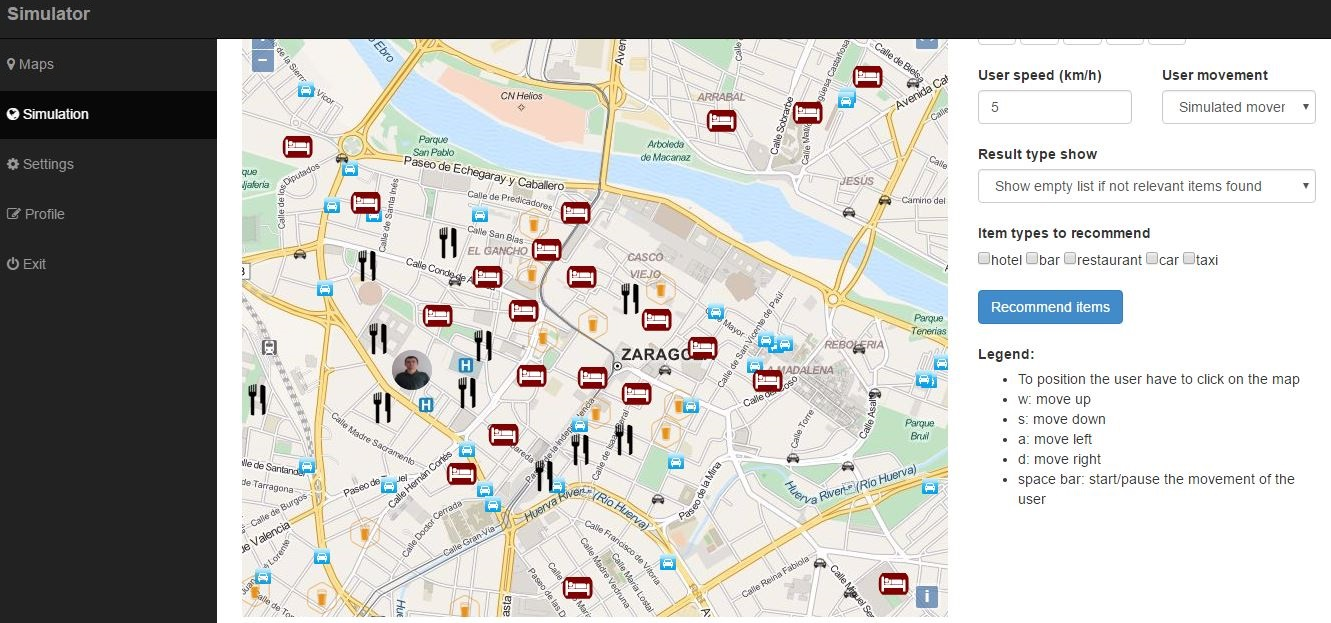
\includegraphics[width=0.55\textwidth]{imagenes/resumen-simulador.jpg}}
\subfloat[Errores cometidos por el sistema de recomendación]{
	\label{evaluacionEnAccion}
	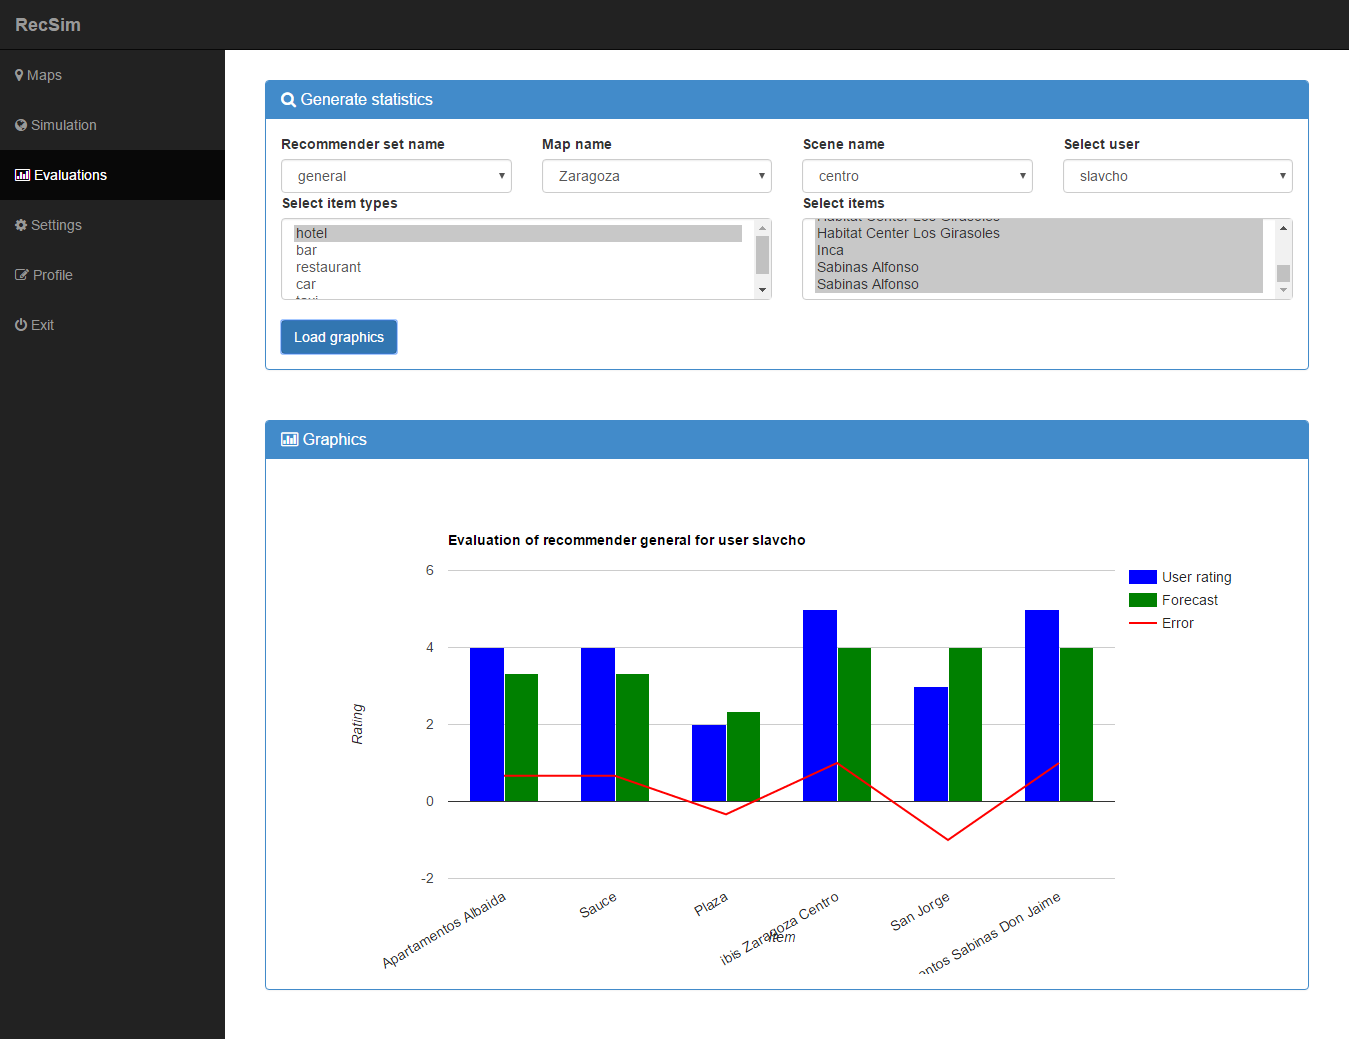
\includegraphics[width=0.35\textwidth]{imagenes/capitulo12/evaluacion.png}}
\caption{Simulador RecSim}
\label{recSim}
\end{figure}

\section{Análisis de requisitos}

\subsection{Requisitos no funcionales}

\begin{table}[H]
	\begin{center}
		\begin{tabular}{|p{1.5cm}| p{10.5cm}|}
			\hline
			Código & Descripción \\
			\hline
			RNF-1  & La aplicación tratara de un simulador. Dicha simulación se realizara sobre mapas online\\ \hline
			RNF-2  & La navegación por los menús de la aplicación se realizara mediante una interfaz gráfica\\ \hline
			RNF-3  & Los textos por defecto de la aplicación serán en inglés\\ \hline
			RNF-4  & La autenfiticación de usuarios se realizará mediante web tokens\\ \hline
			RNF-5  & La interfaz gráfica debe ser responsive desarrollada con bootstrap\\ \hline
			RNF-6  & El back-end debe ser desarrollado con node.js, sockets.io y express \\ \hline
			RNF-7  & El front-end debe ser desarrollado con Angular.js\\ \hline
		\end{tabular}
		\caption{Requisitos no funcionales}
		\label{tabla:requisitosNoFuncionales}
	\end{center}
\end{table}

\newpage

\subsection{Requisitos funcionales}


\begin{longtable}[H]{|c|p{10cm}|}
	% aquí añadimos el encabezado de la primera hoja.
	\hline
	Código & Descripción \\
	\hline \hline
	\endfirsthead
	
	% aquí añadimos el encabezado del resto de hojas.
	\hline
	Código & Descripción \\
	\hline \hline
	\endhead
	
	% aquí añadimos el fondo de todas las hojas, excepto de la última.
	\multicolumn{2}{c}{}
	\endfoot
	
	% aquí añadimos el fondo de la última hoja.
	\endlastfoot
	
	% aquí añadimos el cuerpo de la tabla.
	RF-1  & La aplicación permitirá crear un nuevo usuario\\ \hline
	RF-2  & La aplicación permitirá al usuario buscar mapas por su nombre, tipo, estado, cuidad y fecha de creación\\ \hline
	RF-3  & La aplicación permitirá al usuario crear un nuevo mapa\\ \hline
	RF-4  & La aplicación permitirá al usuario crear una nueva escena asociada a un mapa existente\\ \hline
	RF-5  & La aplicación listara todas las escenas de un mapa\\ \hline
	RF-6  & La aplicación permitirá al usuario editar un mapa existente\\ \hline
	RF-7  & La aplicación permitirá al usuario editar las escenas de un mapa existente\\ \hline
	RF-8  & La aplicación permitirá al usuario crear un nuevo tipo de objeto estático\\ \hline
	RF-9  & La aplicación permitirá al usuario crear un nuevo tipo de objeto dinámico\\ \hline
	RF-10 & La aplicación listará todos los tipos de objetos estáticos creados\\ \hline
	RF-11 & La aplicación listará todos los tipos de objetos dinámicos creados\\ \hline
	RF-12 & La aplicación permitirá al usuario editar los objetos estáticos credos\\ \hline
	RF-13 & La aplicación permitirá al usuario editar los objetos dinámicos creados\\ \hline
	RF-14 & La aplicación permitirá al usuario cambiar el nombre\\ \hline
	RF-15 & La aplicación permitirá al usuario cambiar su contraseña\\ \hline
	RF-16 & La aplicación permitirá al usuario cambiar la imagen asociada a un usuario\\ \hline
	RF-17 & La aplicación permitirá al usuario configurar un nuevo tipo de recomendador\\ \hline
	RF-18 & La aplicación permitirá al usuario editar la configuración de recomendador existente\\ \hline
	RF-18 & La aplicación permitirá al usuario asociar un recomendador existente a una escena\\ \hline
	RF-19 & La aplicación permitirá al usuario definir los limites de una escena\\ \hline
	RF-20 & La aplicación permitirá al usuario asociar un objeto estático a una escena\\ \hline
	RF-21 & La aplicación permitirá al usuario cargar todos los objetos estáticos desde un fichero JSON\\ \hline
	RF-22 & La aplicación permitirá asociar un objeto dinámico y su definir su ruta en una escena\\ \hline
	RF-23 & La aplicación permitirá al usuario cargar todos los objetos dinámicos y sus rutas desde un fichero JSON\\ \hline
	RF-24 & La aplicación listará todos objetos estáticos asociados a una escena \\ \hline
	RF-25 & La aplicación listará todos los objetos dinámicos asociados a una escena \\ \hline
	RF-26 & La aplicación permitirá borrar un objeto estático asociado a una escena\\ \hline
	RF-27 & La aplicación permitirá borrar un objeto dinámico asociado a una escena\\ \hline
	RF-28 & La aplicación permitirá al usuario elegir un si mapa es colaborativo o no\\ \hline
	RF-29 & La aplicación permitirá al usuario ejecuta una simulación sobre la escena de un mapa\\ \hline
	RF-30 & La aplicación permitirá al usuario solicitar recomendaciones mientras se está ejecutando una simulación siempre y cuando el recomendador asociado a la escena es de tipo pull\\ \hline
	RF-31 & El usuario recibirá recomendaciones sin haberlas solicitado siempre y cuando el recomendador asociado a la escena de es tipo push\\ \hline
	RF-32 & El usuario puede arrancar/pausar una simulación\\ \hline
	RF-33 & La aplicación permitirá al usuario generar de forma aleatoria los grafos de movimiento de los vehículos \\ \hline	
	\caption{Requisitos funcionales}
	\label{tabla:requisitosFuncionales}
\end{longtable}

\newpage

\section{Arquitectura del sistema}

La arquitectura del sistema consta de cliente o navegador web, servidor web Node.js, servidor de recomendaciones y base de datos mongoDB (figura \ref{arquitecturaComponentes}).

El la figura \ref{arquitecturaComponentes} observamos que el navegador web se conecta al servidor Node.js mediante dos maneras: la primera es HTTP y la segunda es un sistema bidireccional dirigido por eventos. Las funcionalidades como creación de escenas, búsqueda de mapas etc. están desarrollados sobre una REST API y el intercambio de mensajes JSON.

El sistema bidireccional dirigido por eventos es utilizado  durante la simulación por una parte para reflejar los eventos generados por un usuario al resto de usuarios, y por otra para integrar el navegador, el servidor Node.js y el recomendador. De esta manera conseguimos compartir información entre los distintos componentes sin que estos los hayan solicitado evitando muchas peticiones innecesarias.

\begin{figure}[H]
\centering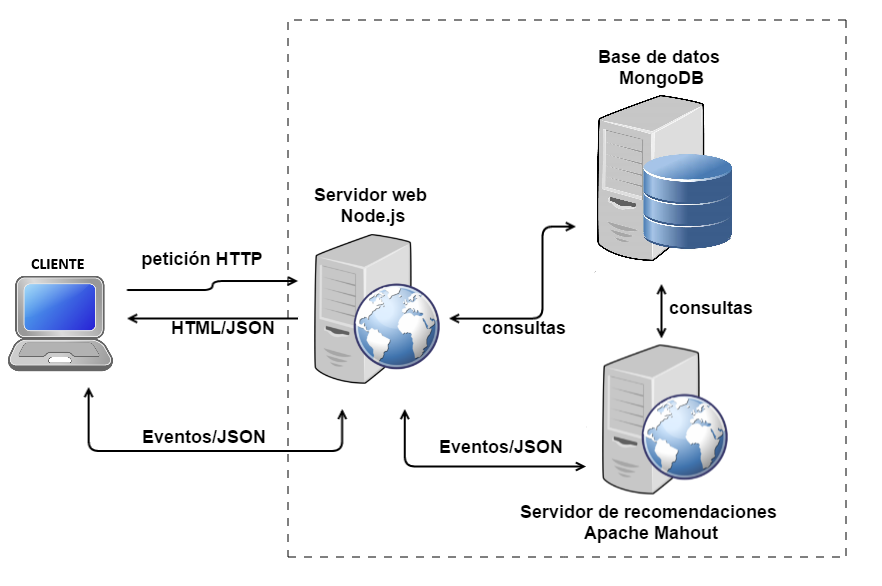
\includegraphics[scale=0.4]{imagenes/arquitectura-componentes.png}
\caption{Arquitectura de componentes del sistema}
\label{arquitecturaComponentes}
\end{figure}

\newpage

\subsection{Arquitectura del front-end}

Para el desarrollo del front-end se han utilizado los frameworks Angular.js y bootstrap. Se ha decidido utilizar estas tecnologías porque nos ofrece varias ventajas: ahorro de recursos, mejora de la productividad y la posibilidad de realizar una simulación sobre dispositivos móviles con el mismo código fuente.

La arquitectura del front-end está basada en el patrón Modelo-Vista-Controllador de tal forma que para cada vista existe un controlador que contiene la lógica de negocio de esta. El controlador también es el encargado de establecer comunicación con el back end. Esta comunicación se realiza entre los llamados Servicios\footnote{es pequeña fabrica de funciones y objetos inyectada en los controladores} de Angular.js y la REST API del back end. Los Servicios de Angular.js son muy necesarios y útiles ya que nos permiten crear un envoltorio sobre la REST API que nos ofrece el back end y de esta forma centralizar las llamas a la API.

\begin{figure}[H]
\centering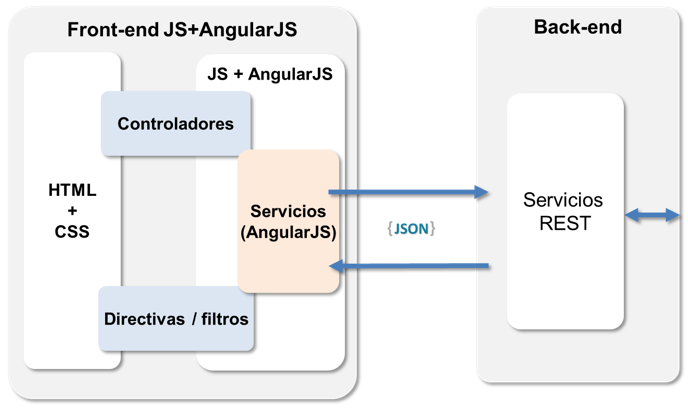
\includegraphics[scale=0.5]{imagenes/arquitectura-front-end.png}
\caption{Arquitectura del front-end}
\label{arquitecturaFrontEnd}
\end{figure}

\subsection{Arquitectura del back-end}

Para el desarrollo del back-end se han utilizado Node.js\footnote{javascript al lado del servidor}, Express\footnote{modulo de Node.js que nos ofrece la posibilidad de desarrollar una REST API}, socket.io\footnote{sistema bidireccional dirigido por eventos} y mongoose \footnote{modelado de objetos sobre mongoDB}. Se ha decidido utilizar estas tecnología por que nos ofrecen las siguientes ventajas: mejora la productividad a la hora de desarrollar el back-end, nos permite desarrollar un back-end ligero que consuma pocos recursos y el modulo sockets.io nos ofrece la posibilidad de desarrollar un sistema bidireccional dirigido por eventos.


\newpage

La arquitectura del back-end se basa en la filosofía de desarrollo de aplicaciones con Node.js y Express y consiste de la siguiente estructura de directorios:

\dirtree{%
.1 Simulator.
.2 app.js.
.2 package.json.
.2 bin.
.3 www.
.2 models.
.2 public.
.3 images.
.3 javascript.
.4 angular.
.4 bootstrap.
.4 jquery.
.4 openlayers.
.4 socketIO.
.3 stylesheets.
.3 views.
.4 configurations.
.4 maps.
.4 settings.
.4 index.html.
.4 register.html.
.3 index.html.
.2 routes.
.3 configuratios.js.
.3 maps.js.
.3 simulation.js.
.3 user.js.
}

\newpage

A continuación vamos a ver más detalladamente cual es la función de cada elemento de este directorio:
\begin{itemize}
	\item app.js: centraliza las configuraciones de nuestra aplicación como por ejemplo en que puerto arranca el servidor, establecer conexiones con la base de datos, configuraciones del router\footnote{el router de Node.js es el encargado del direccionamiento de las peticiones y hace referencia a la definición de puntos finales de aplicación (URI) y cómo responden a las solicitudes de cliente} etc.
	\item package.json: es un gestor de paquetes y contiene los módulos que se están utilizando en nuestra aplicación.
	\item public: es un directorio que contiene la parte visual, es decir el front-end. Podemos ver que este contiene varios subdirectorios:
	\begin{itemize}
	\item en images se ubican las imágenes o iconos usados en la aplicación.
	\item en javascript se ubican los frameworks Javascript usados en en el front-end como Angular.js, Bootstrap, OpenLayers etc. En el subdirectorio angular podemos encontrar las configuraciones de Angular.js, los controladores de las vistas, los Servicios etc.
	\item en views se ubican las vistas del front-end.
	\item en stylesheets están ubicadas las hojas de estilos
	\end{itemize}
	\item en routes se ubican las distintas rutas de Express. En nuestro caso tenemos una para cada menú de la aplicación. Por ejemplo todas las operaciones referentes al menú Maps se encuentra en el fichero maps.js etc.
\end{itemize}

\subsection{Arquitectura de recomendador}

El desarrollo del recomendador está realizado con Java 7, la librería Apache Mahout y socket.io-client. El recomendador desarrollado es un recomendador pull\footnote{tipo de recomendador en el cual los usuarios solicitan recomendaciones} de ejemplo basado en los usuarios (User based recommender). 

Aunque sea un recomendador de ejemplo este está pensado para se expandido, tanto para otro tipo de recomendadores (como pueden ser los recomendadores de tipo push\footnote{tipo de recomendador que realiza recomendaciones sin que el usuario los haya solicitado}) como para la implementación de nuevos tipos de estrategias para el recomendador de tipo pull.

Durante el arranque el servidor del recomendador lanza un hilo por cada tipo de recomendador. En nuestro caso solo lanza un hilo que se corresponde al servidor de tipo pull. Este hilo es el que contiene los eventos que invoca el simulador de escenarios. En la figura \ref{diagramaEventos} observamos que tenemos solo dos eventos: uno para recuperar los tipos de implementaciones\footnote{en nuestro caso es User based recommender pero existen otros tipos como Item based recommender} y otro para realizar las recomendaciones.

\begin{figure}[H]
\centering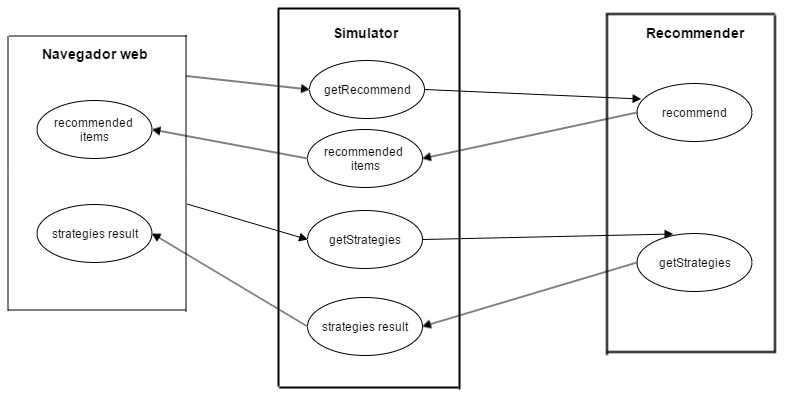
\includegraphics[scale=0.5]{imagenes/diagrama-de-eventos.png}
\caption{Diagrama de eventos}
\label{diagramaEventos}
\end{figure}

El evento recommend es el que se dispara cuando uno de los usuarios solicita una recomendación. Para que se puedan utilizar distintos tipos de implementaciones del recomendador de tipo pull se ha implementado un patrón de diseño de tipo Strategy. Este patrón de diseños nos permite cambiar de estrategia de recomendación en tiempo de ejecución:

\begin{figure}[H]
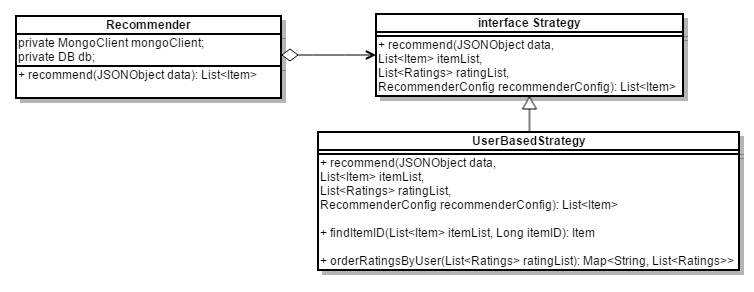
\includegraphics[scale=0.65]{imagenes/uml.png}
\caption{Diagrama uml del patrón de diseño de tipo Strategy}
\label{diagramaUMLStrategy}
\end{figure}

\subsection{Autentificación basada en token}

La autentificación es una de las partes más importantes de un sistema. En este desarrollo se ha optado por una autentificación basada en token. En la autentificación basada en token, las cookies y las sesiones no se utilizan. Se emplea un token para autentificar al usuario en cada petición que se hace al servidor. El flujo de control es el siguiente:
\begin{enumerate}[1.]
	\item el usuario provee un nombre de usuario y contraseña en el formulario de login.
	\item una vez hecha la petición, se valida el usuario en el back-end mediante una consulta a la base de datos. Si la petición es válida, se crea un token utilizando la información de usuario brindada por la base de datos, y luego se retorna esa información en el encabezado de la respuesta, para así guardar el token en almacenamiento local.
	\item se provee la información del token en el encabezado de cada petición para acceder a endpoints restringidos de la aplicación.
	\item si el token tomado del encabezado de la petición es válido, se permite al usuario acceder al endpoint especificado, y se responde con JSON o HTML.
\end{enumerate}

\begin{figure}[H]
	\centering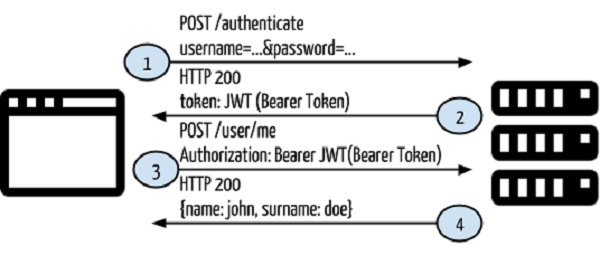
\includegraphics[scale=0.7]{imagenes/token.png}
	\caption{Autentificación Basada en Token}
	\label{token}
\end{figure}

\newpage

\subsubsection{Estructura de un token}

Un token consiste de tres partes:
\begin{itemize}
	\item encabezado: es la parte del token que almacena el tipo de token y el método de encriptación, que a su vez está encriptado en base-64.
	\item carga útil: incluye la información que queremos encriptar.
	\item firma: consiste de combinaciones del encabezado, carga útil, y clave secreta. La clave secreta debe ser almacenada del lado servidor.
\end{itemize}

\begin{figure}[H]
	\centering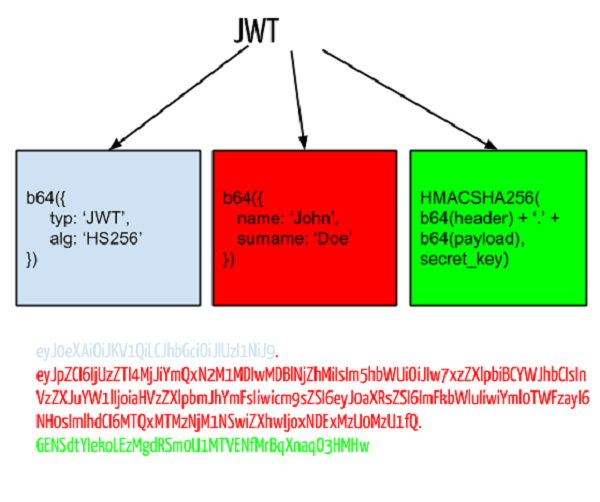
\includegraphics[scale=0.5]{imagenes/jwt.png}
	\caption{Formato del Token}
	\label{formatoToken}
\end{figure}

\section{Menús del simulador de escenarios}

Como en todas las aplicaciones, el simulador de escenarios cuenta con un sistema de menús que dan acceso a las distintas opciones del simulador. En este caso se ha seguido la paradigma WIMP para la organización de los menús y distintas opciones (figura \ref{mapaNavegacion}). Existen 4 tipos de caminos organizados en forma de árbol:

\begin{itemize}
	\item busqueda y gestión (creación, edición y borrados) de mapas y escenas
	\item simulación de un mapa y escena
	\item gestión de tipos de recomendadores, objetos estáticos\footnote{objetos que no cambian de posición a medida que pasa el tiempo} y dinámicos\footnote{objetos que cambian de posición a medida que pasa el tiempo. Tienen una ruta definida durante la creación de la escena}
	\item configuraciones del perfil del usuario
\end{itemize} 

\begin{figure}[H]
\centering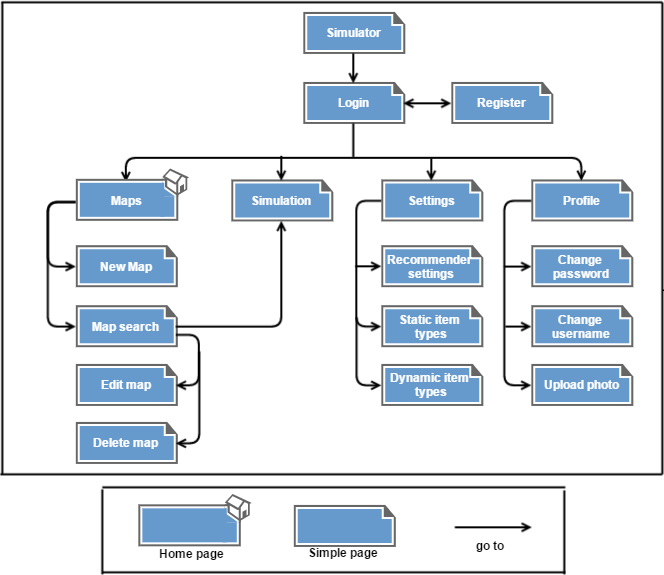
\includegraphics[scale=0.7]{imagenes/mapa-navegacion.png}
\caption{Mapa de navegación}
\label{mapaNavegacion}
\end{figure}

\newpage

\section{Navegación por estima}

La navegación por estima es una técnica que se aplica en el cliente. Consiste en procesar en cada ciclo el estado de los objetos móviles. Se trata de una técnica analítica utilizada en la náutica para la navegación y situación de los barcos y se tienen en cuenta los siguientes elementos: la situación actual, rumbo y velocidad. Es decir, sabiendo la velocidad, el rumbo de la nave y el tiempo transcurrido se puede estimar la posición de la misma al cabo del tiempo. 

Con este método conseguimos calcular cual es la siguiente posición geográfica donde tenemos que colocar un objeto móvil al acabo de un tiempo (el tiempo de refresco de la pantalla). Como ventaja conseguimos disminuir el error en el cálculo de las posiciones de los objetos móviles. Así obtenemos movimientos muy precisos incluso en grafos de movimientos con nodos muy cercanos.

%\section{Explotación del simulador}

%Un usuario nuevo entra en el simulador y visita y valora una serie de items como por ejemplo restaurantes. Al hacer click sobre el item se muestra información relevante del item. El usuario valorará el item en función de estos atributos u otros factores que el considere importantes. A partir de estas valoraciones se evalúa que otros items se le recomiendan al usuario por el recomendador. 

%A continuación vamos a ver si las recomendaciones ofrecidas tienen sentido, es decir, el simulador va calculando los errores. Para cuantificar el error se ha utilizado la métrica Medium Absolute Error (MAE). La MAE consiste en restar la valoración del usuario del valor estimado del recomendador. Hacemos pruebas con varios usuarios y sacamos medias de su satisfacción con el sistema de recomendación.

%\newpage

%\begin{figure}[H]
%	\centering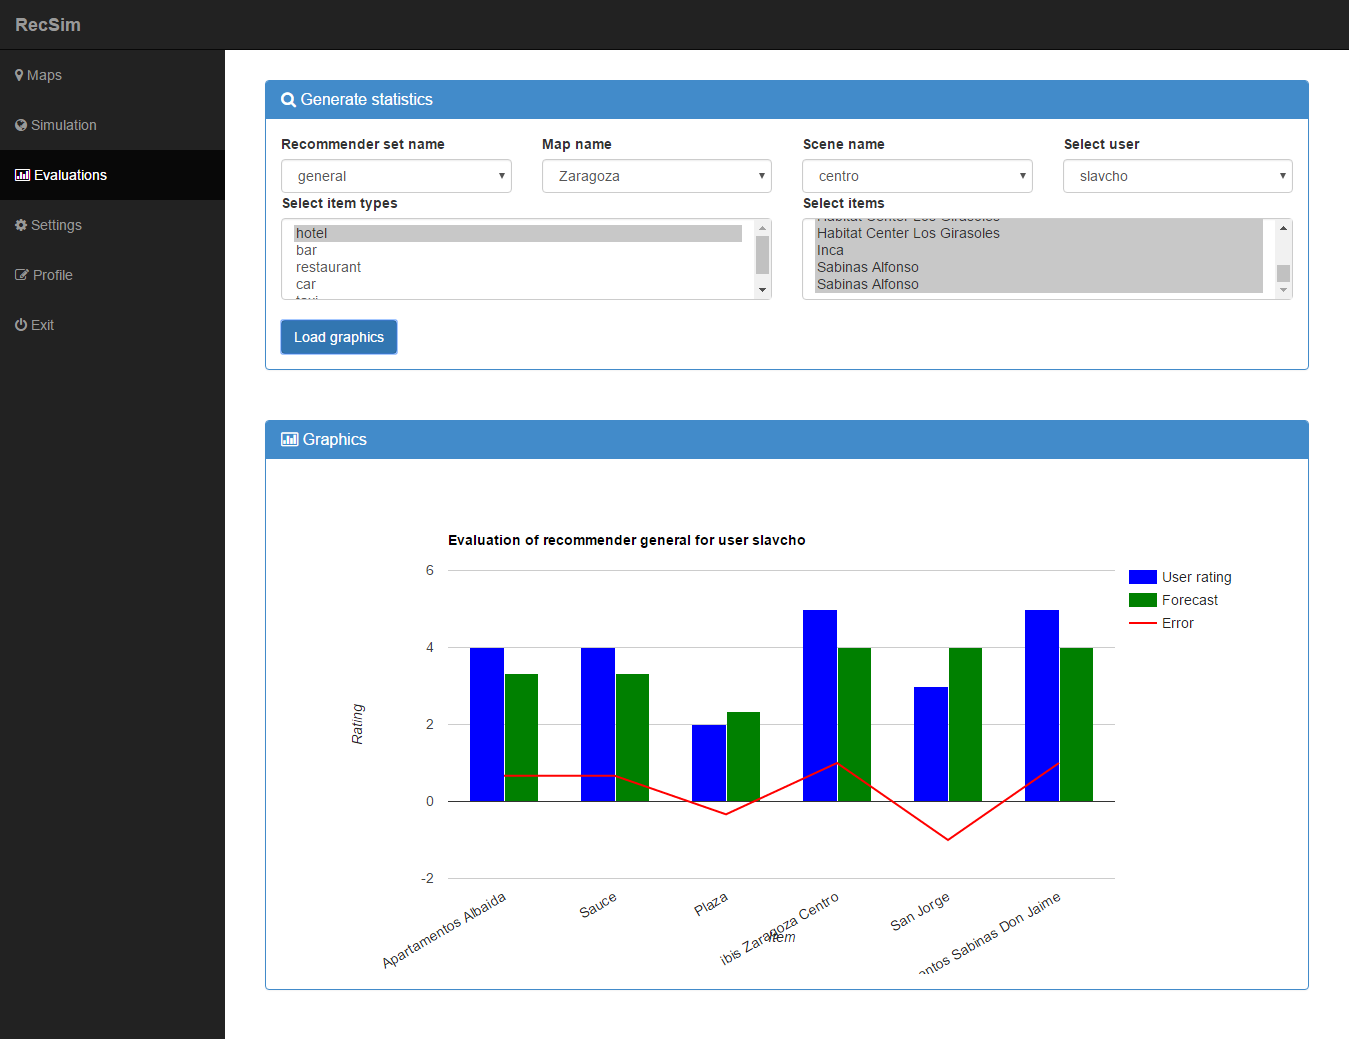
\includegraphics[scale=0.35]{imagenes/capitulo12/evaluacion.png}
%	\caption{Evaluación de un recomendador}
%	\label{evaluacionRecomendador}
%\end{figure}
%w
\chapter{Gestión del proyecto}


En este capítulo se explican el modelo de proceso seleccionado y las distintas etapas por las que ha pasado el este Trabajo Fin de Grado centradose únicamente en los aspectos más importantes. Para profundizar más sobre estos aspectos debe acudir a los anexos.

\section{Modelo de proceso seleccionado}


Este Trabajo Fin de Grado ha surgido una importante evolución desde el primer planteamiento hasta la obtención del sistema final. La primera idea para la evaluación de los algoritmos de recomendaciones era la utilización de un videojuego ya que este podría recolectar datos de forma transparente mientras los usuarios se divertian. El videojuego consistiría en el cumplimiento de misiones en una cuidad basandose en algún videojuego de aventuras como el videojuego Paperboy del año 1985 donde un chico reparte periódicos en una cuidad.

Por esto se ha planteado usar el motor gráfico Unity 5 para el desarrollo del videojuego ya que no tenía sentido desarrollar un videojuego usando simplemente un lenguaje de programación. Pero existía la incertidumbre si todos los requisitos podrían ser implementados. Esto era debido porque por una parte no se conocían de antemano todos los requisitos y por otra no se conocía si el motor gráfico tenía algún tipo de limite. 

Para solucionar estos problemas se ha tomado la decisión de elegir el modelo en espiral como modelo de trabajo. Las actividades de este modelo forman una espiral de tal forma que cada iteración representa un conjunto de actividades. Esto nos permitiría segmentar el trabajo en tareas más pequeñas e ir definiendo los requisitos mientras se desarrollaba el videojuego. De esta manera podríamos evaluar si los requisitos propuestos podrían o no ser implementados con Unity 5. En caso de que el motor gráfico tuviese algún límite tendríamos la capacidad de reorientar el proyecto.

\subsection{Etapa 1}

En la tabla \ref{tabla:requisitosEtapa1} podemos encontrar las tareas que han sido definidas para esta etapa:

\begin{table}[H]
\begin{center}
\begin{tabular}{|p{1.5cm}| p{10.5cm}|}
\hline 
Código & Descripción \\
\hline \hline
RQ-0  & Formación básica con Unity 5\\ \hline
RQ-1  & Establecer puntos en el mapa para que el jugador pueda ir a buscarlos. \\ \hline
RQ-2  & Los puntos establecidos en el requisitos RQ-1 deben de ser extraibles desde un servidor externo\\ \hline
RQ-3  & Establecer una conexión HTTP/JSON entre Unity 5 y un servidor externo. \\ \hline
RQ-4  & Sacar el modelado geométrico de un servidor externo \\ \hline
RQ-5  & El videojugo debe de tener un menú principal \\ \hline
RQ-6  & Investigar si se puede usar Longitud y Latitud con Unity 5 \\ \hline
RQ-7  & Investigar si los edificio generados con CityEngine 2014 son reales o no \\ \hline
RQ-8  & Permitir que el juego se realice sobre mapas de ciudades reales \\ \hline
RQ-9  & Investigar si es posible el desarrollo de videojuego en 3D \\ \hline
\end{tabular}
\caption{Tareas etapa 1}
\label{tabla:requisitosEtapa1}
\end{center}
\end{table}

Como conclusión de esta etapa obtenemos el siguiente resultado:
\begin{itemize}
	\item puede establecerse una conexión con un servidor externo mediante HTTP/JSON (RQ-3). 
	\item pueden establecerse puntos en el mapa para que el jugador pueda ir a buscarlos(RQ-1). 
	\item pueden extraerse puntos desde un servidor externo para que el usuarios pueda ir a buscarlos (RQ-1 y RQ-3).
	\item la realizacion del menú principal del videojuego ha sido posible.
	\item Unity 5 utiliza eje de abscisas. Por lo tanto si queremos usar coordenadas geográficas tenemos que calcular la Longitud y Latitud a partir del eje de coordenadas (x, y, z).
	\item los datos sobre los edificios de OpenStreetMap no están completos.
	\item se ha decido de dejar atrás el modelado 3D ya que se han detectado los siguientes problemas: coste en cuanto a tiempo demasiado grande para el diseño de una ciudad, CityEngine 2014 no interpreta correctamente los datos exportados además no existe ninguna otra herramienta que nos permita la correcta interpretación de los datos (por lo menos yo no podido encontrarla).
\end{itemize}

\subsection{Etapa 2}

En la tabla \ref{tabla:requisitosEtapa2} podemos encontrar las tareas que han sido definidas para esta etapa:

\begin{table}[H]
\begin{center}
\begin{tabular}{|p{1.5cm}| p{10.5cm}|}
\hline 
Código & Descripción \\
\hline \hline
RQ-10 & Investigar como se desarrollan grafos en Unity para la posterior implementación de la IA sobre estos para el movimiento de los vehículos etc. \\ \hline
RQ-11 & Diseñar y desarrollar un mapa del juego\\ \hline
\end{tabular}
\caption{Tareas etapa 2}
\label{tabla:requisitosEtapa2}
\end{center}
\end{table}

Como conclusión de esta etapa obtenemos el siguiente resultado:
\begin{itemize}
	\item Unity 5 dispone de su propio modulo de IA y por lo tanto no hace falta implementar algoritmos de IA para el comportamiento de los objetos dinámicos.
	\item en esta etapa se ha definido el requisito que el juego tiene que funcionar sobre cualquier mapa del mundo. Por lo tanto en la siguiente etapa hay que investigar si es posible la integración de Unity 5 con OpenStreetMap.
\end{itemize}

\newpage

\subsection{Etapa 3}

En la tabla \ref{tabla:requisitosEtapa3} podemos encontrar las tareas que han sido definidas para esta etapa:

\begin{table}[H]
\begin{center}
\begin{tabular}{|p{1.5cm}| p{10.5cm}|}
\hline 
Código & Descripción \\
\hline \hline
RQ-11 & Investigar en que consiste el formato OSM\\ \hline
RQ-12 & Investigar si es posible la integración de OpenStreetMap con Unity\\ \hline
\end{tabular}
\caption{Tareas etapa 3}
\label{tabla:requisitosEtapa3}
\end{center}
\end{table}

Como conclusión de esta etapa obtenemos el siguiente resultado:
\begin{itemize}
	\item Unity 5 no puede ser integrado con OpenStreetMap y no es capaz de renderizar mapas a partir sus datos (ficheros OSM). 
	\item en esta etapa se ha decido reorientar el proyecto por las siguientes razones: Unity 5 no puede ser integrado con OpenStreetMap por lo tanto la única opción para desarrollar un videojuego sobre mapas reales es desarrollando el videojuego desde cero con algún lenguaje como Java y el inconveniente que esto representa es que es demasiado costoso en cuanto a tiempo y dificultad.  
\end{itemize}

\subsection{Etapa 4}

En la tabla \ref{tabla:requisitosEtapa4} podemos encontrar las tareas que han sido definidas para esta etapa:

\begin{table}[H]
\begin{center}
\begin{tabular}{|p{1.5cm}| p{10.5cm}|}
\hline 
Código & Descripción \\
\hline \hline
RQ-12 & instalar mongoDB\\ \hline
RQ-13 & instalar Node.js y NPM\\ \hline
RQ-14 & instalar git\\ \hline
RQ-14 & instalar Java y Apache maven\\ \hline
RQ-16 & Desarrollar y configurar la base de la aplicación con Node.js\\ \hline
RQ-17 & Instalar y configurar Angular.js\\ \hline
RQ-18 & Instalar y configurar OpenLayers.js\\ \hline
RQ-19 & Instalar y configurar Bootstrap\\ \hline
\end{tabular}
\caption{Tareas etapa 4}
\label{tabla:requisitosEtapa4}
\end{center}
\end{table}

\newpage

Como conclusión de esta etapa obtenemos el siguiente resultado:
\begin{itemize}
	\item se han instalado y configurado todas las herramientas y frameworks necesarios para el desarrollo de la aplicación.
\end{itemize}

\subsection{Etapa 5}

En la tabla \ref{tabla:requisitosEtapa5} podemos encontrar las tareas que han sido definidas para esta etapa:

\begin{table}[H]
\begin{center}
\begin{tabular}{|p{1.5cm}| p{10.5cm}|}
\hline 
Código & Descripción \\
\hline \hline
RQ-20 & Definir lo requisitos funcionales y no funcionales de la aplicación\\ \hline
RQ-21 & Desarrollar el front-end\\ \hline
RQ-22 & Deseñar la base de datos\\ \hline
RQ-23 & Diseñar y desarrollar el back-end\\ \hline
RQ-24 & Diseñar y desarrollar el recomendador\\ \hline
RQ-25 & Realizar pruebas funcionales de la aplicación\\ \hline
\end{tabular}
\caption{Tareas etapa 5}
\label{tabla:requisitosEtapa5}
\end{center}
\end{table}

Como conclusión de esta etapa obtenemos el siguiente resultado:
\begin{itemize}
	\item la parte mas costosa de esta etapa ha sido la definición de los requisitos de la aplicación.
	\item una vez definidos los requisitos el resto del trabajo ha sido puramente técnico. 
\end{itemize}


\subsection{Etapa 6}

La última etapa consiste en documentar el trabajo realizado en este Trabajo Fin de Grado.

\newpage

\section{Tiempo dedicado}

Como ya se ha comentado anteriormente, el desarrollo del proyecto se ha realizado siguiendo el modelo en espiral. En esta sección se mostrará el tiempo dedicado y también un cronograma de las diferentes etapas.

\begin{table}[H]
\begin{center}
\begin{tabular}{|c|c|}
\hline 
\noindent{\textbf{Fase}} & \noindent{\textbf{Horas}} \\
\hline \hline
Fase 1 & 54\\ \hline
Fase 2 & 6.5\\ \hline
Fase 3 & 38\\ \hline
Fase 4 & 3.5\\ \hline
Fase 5 & 247\\ \hline
Fase 6 & 42.5\\ \hline
Reuniones & 7\\ \hline
Pruebas de carga & 11.5 \\ \hline
\hline \hline
\noindent{\textbf{Total}} & \noindent{\textbf{410}} \\ \hline
\end{tabular}
\caption{Separación por horas de las distintas fases}
\label{tabla:requisitosEtapa5}
\end{center}
\end{table}
 

\begin{figure}[H]
\centering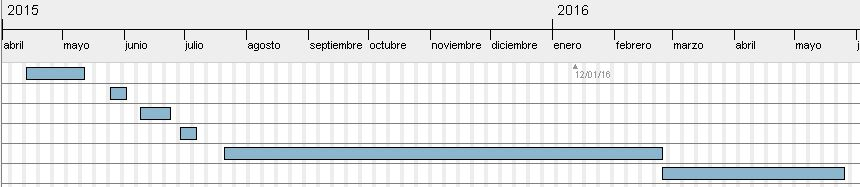
\includegraphics[scale=0.8]{imagenes/gantt.jpg}
\caption{Diagrama de Gantt de las distintas fases del proyecto}
\label{gantt}
\end{figure}

%
\chapter{Conclusiones}

En este capítulo se explican las conclusiones que se han obtenido de este Trabajo Fin de Grado, el trabajo futuro y una valoración personal.

\section{Conclusiones}

A lo largo de este Trabajo Fin de Grado se ha desarrollado un simulador de escenarios con usuarios móviles para la evaluación de algoritmos de recomendaciones. El simulador puede ser usado de forma cooperativa por varias personas a través de cualquier dispositivo con conexión a Internet y un navegador web. Cuenta con escenarios basados en datos reales obtenidos a través del servicio de mapas de OpenStreetMap y permite integrar de un recomendador externo.

Como se puede comprobar a continuación, se han cumplido todos los objetivos marcados inicialmente en la propuesta del Trabajo Fin de Grado:
\begin{itemize}
	\item Se he desarrollado un simulador de escenarios con usuarios móviles que cuenta con mapas de ciudades con objetos móviles y estáticos.
	\item Los mapas de las ciudades utilizados en las simulaciones están creados a partir de datos reales obtenidos a través del servicio de mapas de OpenStreetMap.
	\item Los usuarios puedan crear, editar, borrar y configurar los mapas y escenarios del simulador.
	\item Se ha desarrollado un sistema bidireccional basada en eventos que permite integrar un recomendador externo y realizar simulaciones en tiempo real de tal forma que los eventos de los usuarios se reflejen en los dispositivos conectados al mismo mapa y escena.
\end{itemize}

\section{Trabajos futuros}

A continuación se proponen algunas posibles mejoras futuras:

\begin{itemize}
	\item 
	\item 
	\item 		
\end{itemize}

\section{Valoración personal}


\nocite{*}
\bibliography{bibliografia/bibliografia}\addcontentsline{toc}{chapter}{Bibliografía}
\bibliographystyle{unsrt}
%
%\appendix
%\input{apendices/manual_usuario/manual_usuario}
%%\input{apendices/paper/paper}
%\input{glosario/entradas_glosario}
% \addcontentsline{toc}{chapter}{Glosario}
% \printglossary
\chapter*{}
\thispagestyle{empty}

\end{document}
